%The executive summary is a special chapter before the TOC
% See the other sections (e.g. Context) for more normal chapter headings
%%%%%%%%%%%%%%%%%%%%%%%%%%%%%%%%%%%%
% Call it Front Matter in TOC, as it will include Glossary and auto-generated TOC, LOF.
\chapter[Front Matter]{Executive Summary} 
\label{cha:front}
\addcontentsline{toc}{section}{Executive Summary}
%%%%%%%%%%%%%%%%%%%%%%%%%%%%%%%%%%%%
%Begin the actual executive summary text. If you create any subsections you
%probably want to use  \section*{Section name}  with an asterisk, so they are not numbered.
% Note: to get proper looking quotes use two left/right single quotes: ``. . . ''

%Example of a remark that can be optionally printed:
\begin{remark}\color{blue}
Suggested length of this section: 2 pages including figure(s).
\noindent This the most important section to edit carefully. It should stand alone. Assume it is the \emph{only} section that your corporate liaison's boss will read.
\begin{itemize} \tightlist   % a list with reduced white space
\item Introduce the reader to what your project is about. 
\item Say something brief about the design teams.
\item Motivate the current project direction. The motivation is based on findings from user and expert
interviews, benchmarking, CEP and CFP tests, etc. What interesting findings or insights do you have?
\item \textbf{What you did} is less important than \textbf{what you learned}.
\item Make sure your current ``Point of View'' comes across. The person who reads only the Executive
Summary should still have an idea who your User is.
\item Include one or two images that capture the gist of your design. For Fall, we're probably talking about
pictures of a proposal or vision rather than something you've designed. However, it's possible that something 
from your CFP, CEP or Benchmarking gets the idea across.
\end{itemize}
The remainder of this section is taken from \cite{Autodesk2008Fall}, a pretty good Fall document, done in Latex.
\normalcolor
\end{remark}
%End of remark

%%%%%%%%%%%%%%%%%%BEGIN EXAMPLE TEXT FOR THIS SECTION %%%%%%%%%%%%
\section*{Example text}

Engineers must work with distributed teammates around the world. More than ever, designers are tackling all stages of design with remote coworkers whom they may never actually meet face to face. Functioning in this distributed environment can be very challenging both technically and socially. While there are many great tools for managing data and capturing concepts, sharing the output of these tools between distant teammates requires thoughtful planning and continued effort to include distant coworkers during the meeting. Also, distributed team members often feel a sense of isolation - studies have shown that people will collaborate more with people in the same room than with their distributed coworkers who are calling in \cite{Milnethesis}. Developing a way to level the playing field for distributed designers is essential for ever achieving effective distributed design.

\begin{figure}[h]
	\centering
		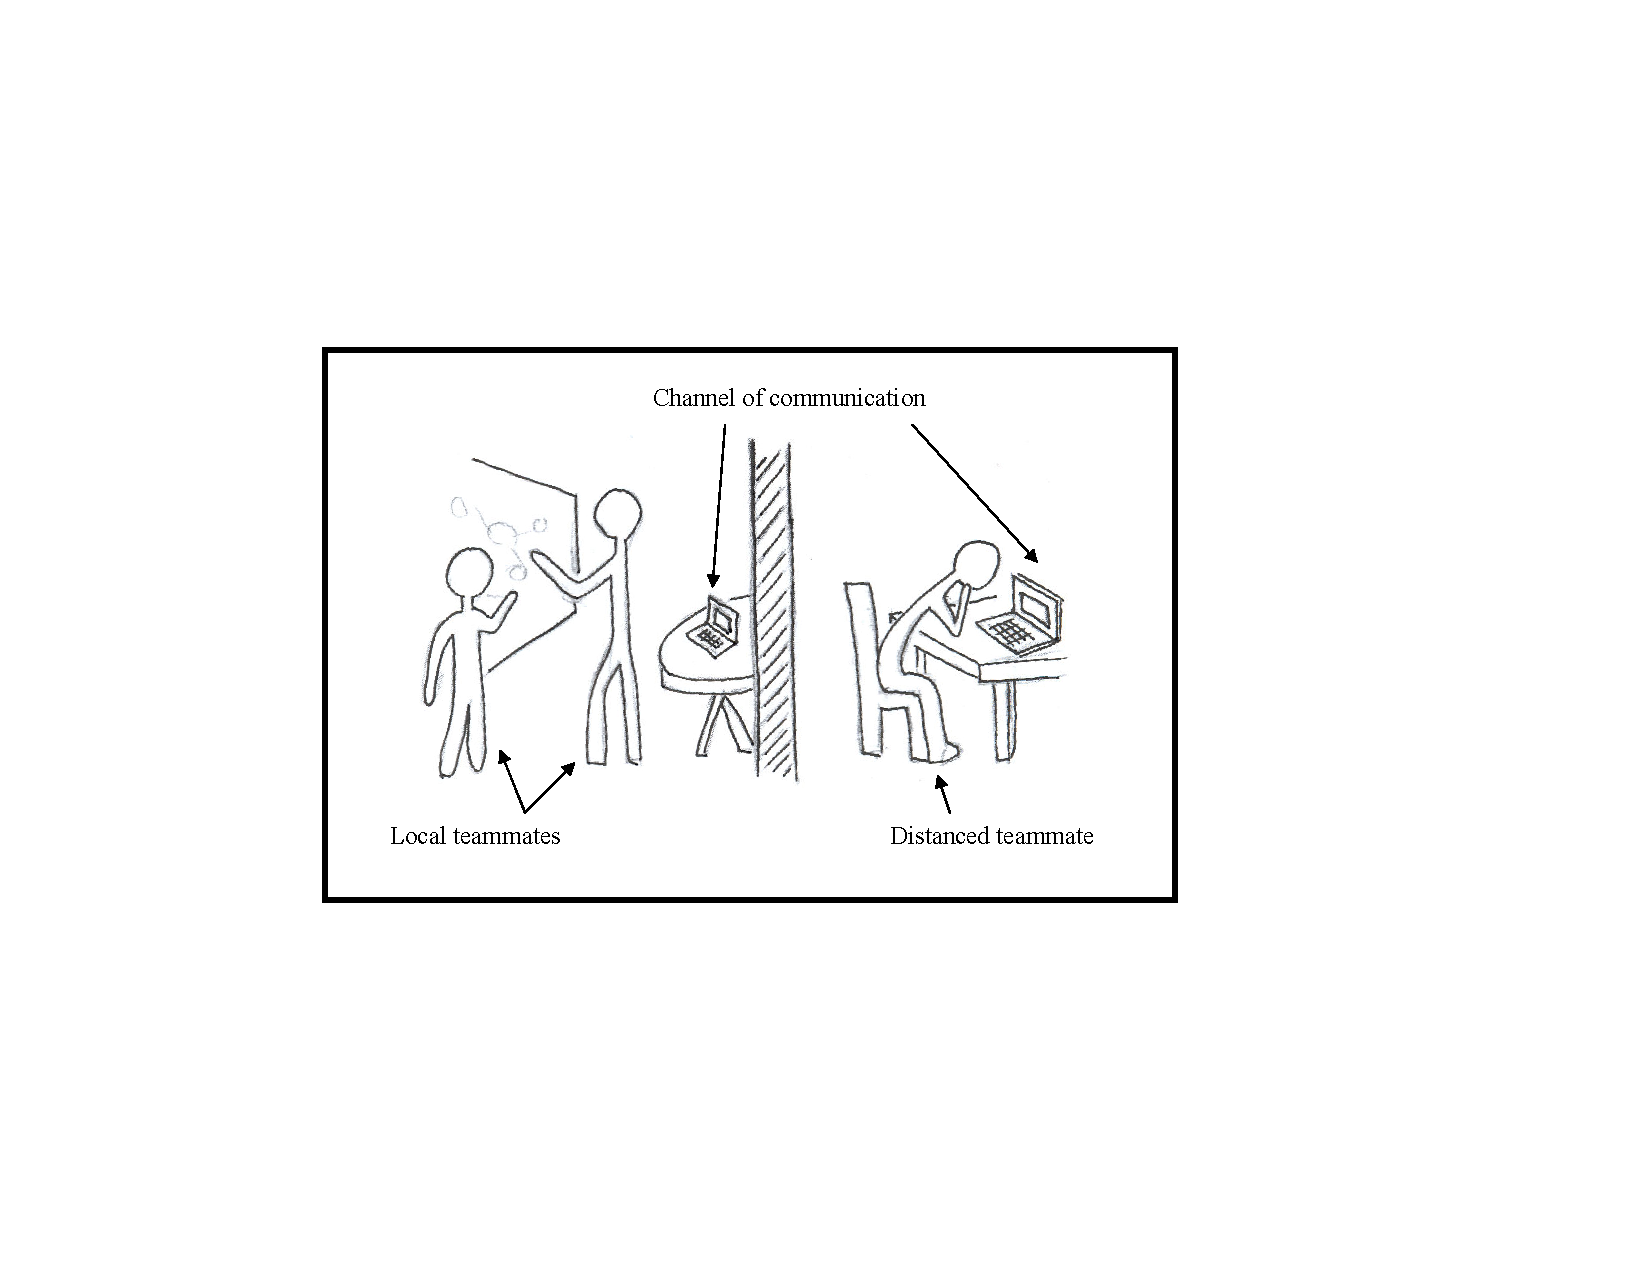
\includegraphics[width=.75\textwidth]{Figures/Ch1frontmatter/execimage.pdf}
	\caption{Common result of destributed design meetings}
	\label{fig:executive}
\end{figure}

 Autodesk has approached our team of 3 engineering students at Stanford University and 3 engineering students at Pontificia Universidad Javeriana to tackle this issue of how to get engineers to collaborate better. To gain an understanding of what makes great collaboration, we have surveyed existing collaboration technology, talked with designers, and run scenarios for different collaboration environments. We focused on solutions for the early stages of the design process between small, distributed teams. 

After researching a plethora of communication devices for sharing audio, displaying video and sharing drawings, we realized that the critical issue was not how to input drawings or video. The more pressing issues are how designers share the output of the tools and how to capture records of the information that is created. During the brainstorming phase, where ideas are generated quickly and randomly, finding a way to record a meaningful and accessible archive of concepts is especially difficult with existing collaboration tools.

Another important component of obtaining improved group collaboration is getting people to work together as a cohesive group, be it a distributed team or not. How do you deal with the coworker who keeps dominating the conversation? How do you get that quiet person to be more involved? No one is responding to my idea, don't they like it? The team has hypothesized that applying one of the key tenants of improvisational acting could assist with these social frustrations - have a moderator. Dialogue is critical to successful brainstorming, and can potentially be facilitated by objective feedback from a third person observer.

We also tested the ability of uncrowded channels to pass information without disturbing the flow of conversation. By prototyping a tactile feedback system, we found that it enabled a non-intrusive way to get someone's attention, and more importantly created a sensation of proximity with distributed teammates. 

\begin{figure}[h]
	\centering
		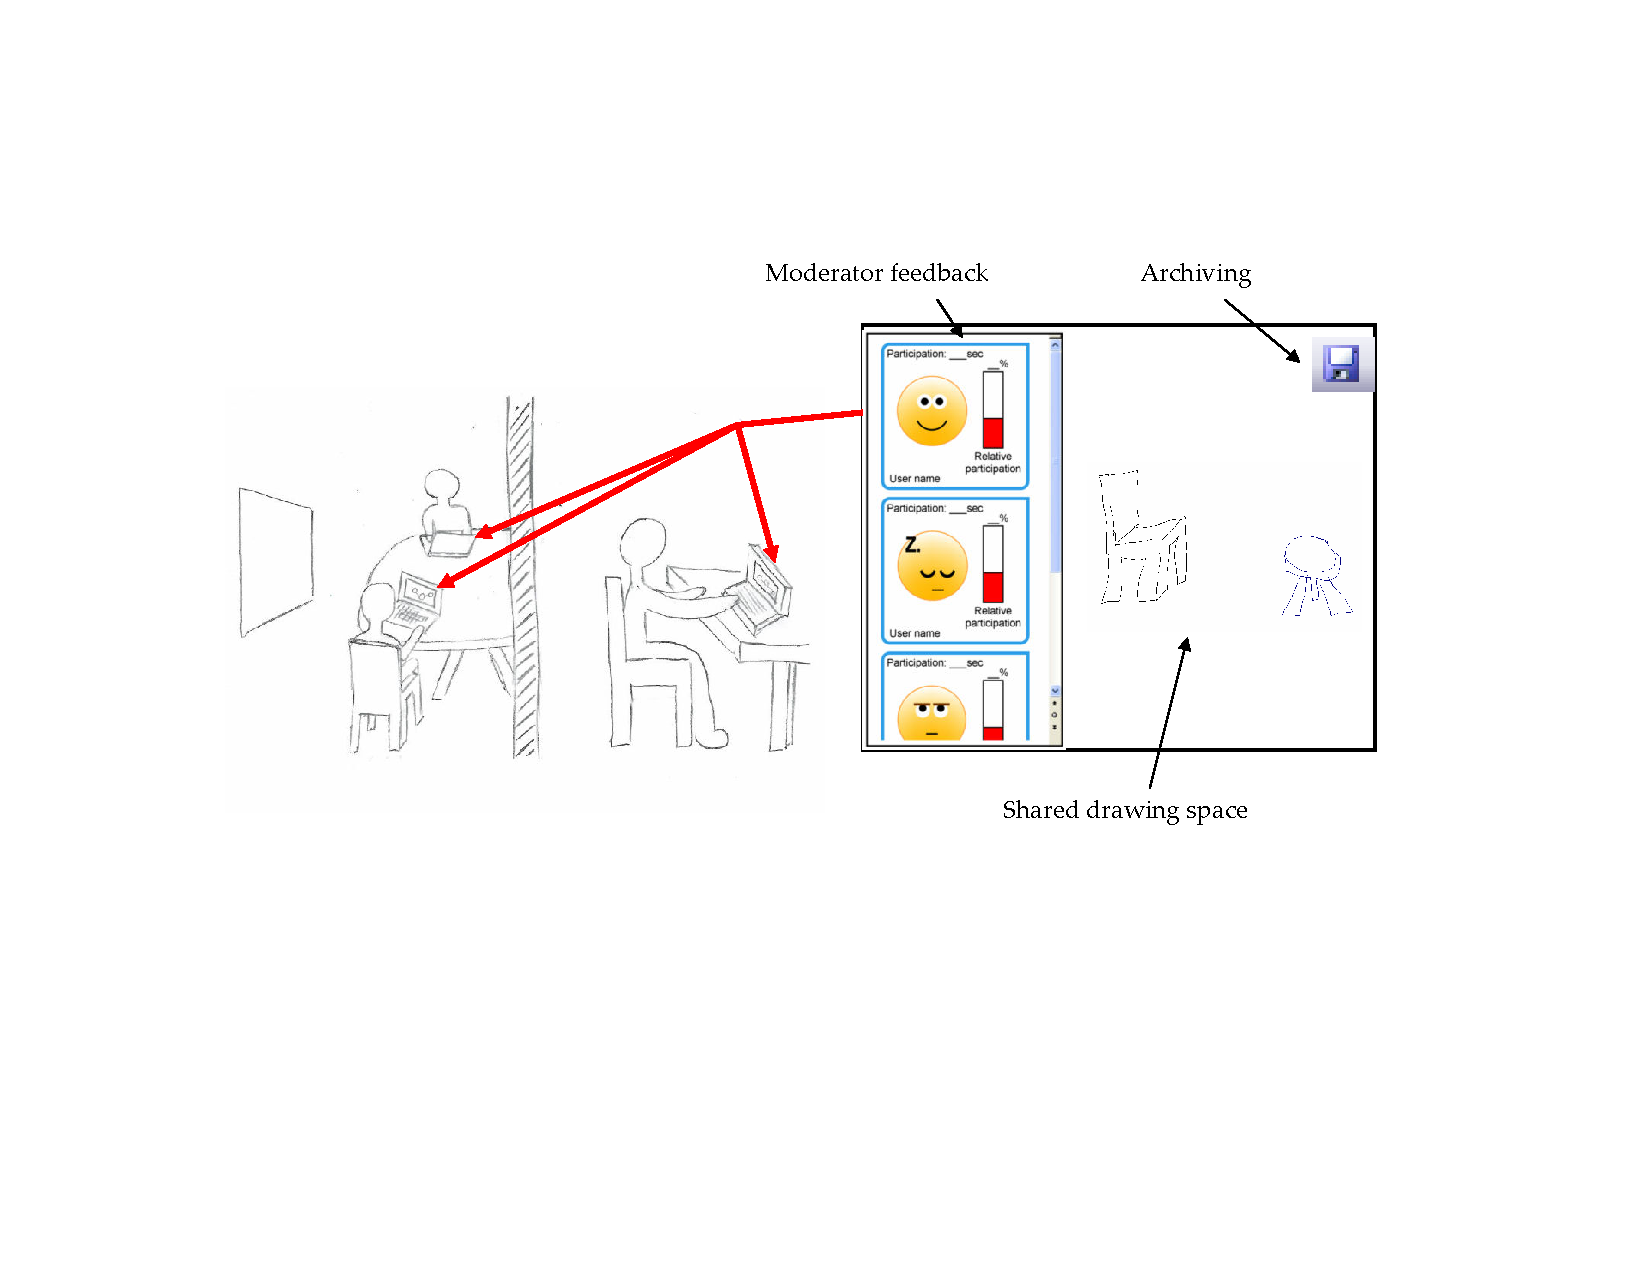
\includegraphics[width=.75\textwidth]{Figures/Ch1frontmatter/execimage2.pdf}
	\caption{Vision for a more effective distributed design meeting}
	\label{fig:execimage2}
\end{figure}

A vision for the final product is to better enable dialogue by displaying explicit teammate feedback and participation level visible to the team. Imagine knowing when someone wasn't paying attention, or that your teammate thought you were talking too much, or that everyone really thinks you're idea is pretty cool. All of this could be displayed without saying anything. Aside from simply providing a platform to share information, the system will monitor the quantity of inputs and determine individual participation level, and also offer the opportunity for direct feedback. The objective is to  provide a real-time answer to a common wonder -  what are my teammates really thinking?  

%%%%%%%%%%%%%%%%%%END EXAMPLE TEXT FOR THIS SECTION %%%%%%%


\begin{remark}\color{blue}
\section*{Latex tips:}
\begin{itemize}\tightlist
\item These remarks in blue disappear if you select \textbackslash commentson\{remark\} in me310report.tex
\item Some teams will find the default report cover sheet too plain and will want to change fonts and layout, etc. This is a tedious in Latex. Use Powerpoint or Photoshop or other program to make a nice outer cover which you can pre-pend to the PDF file from Latex.
\item References are linked using the``cite'' command. The template is currently set up to use a bibliography style sheet ``plainurl310.bst'', which is close to the style used by IEEE and other journals with citation numbers in square brackets (e.g., [1]) and printed alphabetically in the Bibliography section. The modifications provide for printing a URL (if there is one) for each reference in a plain format. Numerous other bibliography styles are available, although many do not work with URLs.
\end{itemize}
\normalcolor \end{remark}
